% Options for packages loaded elsewhere
\PassOptionsToPackage{unicode}{hyperref}
\PassOptionsToPackage{hyphens}{url}
\PassOptionsToPackage{dvipsnames,svgnames,x11names}{xcolor}
%
\documentclass[
  letterpaper,
  DIV=11,
  numbers=noendperiod]{scrreprt}

\usepackage{amsmath,amssymb}
\usepackage{iftex}
\ifPDFTeX
  \usepackage[T1]{fontenc}
  \usepackage[utf8]{inputenc}
  \usepackage{textcomp} % provide euro and other symbols
\else % if luatex or xetex
  \usepackage{unicode-math}
  \defaultfontfeatures{Scale=MatchLowercase}
  \defaultfontfeatures[\rmfamily]{Ligatures=TeX,Scale=1}
\fi
\usepackage{lmodern}
\ifPDFTeX\else  
    % xetex/luatex font selection
\fi
% Use upquote if available, for straight quotes in verbatim environments
\IfFileExists{upquote.sty}{\usepackage{upquote}}{}
\IfFileExists{microtype.sty}{% use microtype if available
  \usepackage[]{microtype}
  \UseMicrotypeSet[protrusion]{basicmath} % disable protrusion for tt fonts
}{}
\makeatletter
\@ifundefined{KOMAClassName}{% if non-KOMA class
  \IfFileExists{parskip.sty}{%
    \usepackage{parskip}
  }{% else
    \setlength{\parindent}{0pt}
    \setlength{\parskip}{6pt plus 2pt minus 1pt}}
}{% if KOMA class
  \KOMAoptions{parskip=half}}
\makeatother
\usepackage{xcolor}
\setlength{\emergencystretch}{3em} % prevent overfull lines
\setcounter{secnumdepth}{5}
% Make \paragraph and \subparagraph free-standing
\makeatletter
\ifx\paragraph\undefined\else
  \let\oldparagraph\paragraph
  \renewcommand{\paragraph}{
    \@ifstar
      \xxxParagraphStar
      \xxxParagraphNoStar
  }
  \newcommand{\xxxParagraphStar}[1]{\oldparagraph*{#1}\mbox{}}
  \newcommand{\xxxParagraphNoStar}[1]{\oldparagraph{#1}\mbox{}}
\fi
\ifx\subparagraph\undefined\else
  \let\oldsubparagraph\subparagraph
  \renewcommand{\subparagraph}{
    \@ifstar
      \xxxSubParagraphStar
      \xxxSubParagraphNoStar
  }
  \newcommand{\xxxSubParagraphStar}[1]{\oldsubparagraph*{#1}\mbox{}}
  \newcommand{\xxxSubParagraphNoStar}[1]{\oldsubparagraph{#1}\mbox{}}
\fi
\makeatother

\usepackage{color}
\usepackage{fancyvrb}
\newcommand{\VerbBar}{|}
\newcommand{\VERB}{\Verb[commandchars=\\\{\}]}
\DefineVerbatimEnvironment{Highlighting}{Verbatim}{commandchars=\\\{\}}
% Add ',fontsize=\small' for more characters per line
\usepackage{framed}
\definecolor{shadecolor}{RGB}{241,243,245}
\newenvironment{Shaded}{\begin{snugshade}}{\end{snugshade}}
\newcommand{\AlertTok}[1]{\textcolor[rgb]{0.68,0.00,0.00}{#1}}
\newcommand{\AnnotationTok}[1]{\textcolor[rgb]{0.37,0.37,0.37}{#1}}
\newcommand{\AttributeTok}[1]{\textcolor[rgb]{0.40,0.45,0.13}{#1}}
\newcommand{\BaseNTok}[1]{\textcolor[rgb]{0.68,0.00,0.00}{#1}}
\newcommand{\BuiltInTok}[1]{\textcolor[rgb]{0.00,0.23,0.31}{#1}}
\newcommand{\CharTok}[1]{\textcolor[rgb]{0.13,0.47,0.30}{#1}}
\newcommand{\CommentTok}[1]{\textcolor[rgb]{0.37,0.37,0.37}{#1}}
\newcommand{\CommentVarTok}[1]{\textcolor[rgb]{0.37,0.37,0.37}{\textit{#1}}}
\newcommand{\ConstantTok}[1]{\textcolor[rgb]{0.56,0.35,0.01}{#1}}
\newcommand{\ControlFlowTok}[1]{\textcolor[rgb]{0.00,0.23,0.31}{\textbf{#1}}}
\newcommand{\DataTypeTok}[1]{\textcolor[rgb]{0.68,0.00,0.00}{#1}}
\newcommand{\DecValTok}[1]{\textcolor[rgb]{0.68,0.00,0.00}{#1}}
\newcommand{\DocumentationTok}[1]{\textcolor[rgb]{0.37,0.37,0.37}{\textit{#1}}}
\newcommand{\ErrorTok}[1]{\textcolor[rgb]{0.68,0.00,0.00}{#1}}
\newcommand{\ExtensionTok}[1]{\textcolor[rgb]{0.00,0.23,0.31}{#1}}
\newcommand{\FloatTok}[1]{\textcolor[rgb]{0.68,0.00,0.00}{#1}}
\newcommand{\FunctionTok}[1]{\textcolor[rgb]{0.28,0.35,0.67}{#1}}
\newcommand{\ImportTok}[1]{\textcolor[rgb]{0.00,0.46,0.62}{#1}}
\newcommand{\InformationTok}[1]{\textcolor[rgb]{0.37,0.37,0.37}{#1}}
\newcommand{\KeywordTok}[1]{\textcolor[rgb]{0.00,0.23,0.31}{\textbf{#1}}}
\newcommand{\NormalTok}[1]{\textcolor[rgb]{0.00,0.23,0.31}{#1}}
\newcommand{\OperatorTok}[1]{\textcolor[rgb]{0.37,0.37,0.37}{#1}}
\newcommand{\OtherTok}[1]{\textcolor[rgb]{0.00,0.23,0.31}{#1}}
\newcommand{\PreprocessorTok}[1]{\textcolor[rgb]{0.68,0.00,0.00}{#1}}
\newcommand{\RegionMarkerTok}[1]{\textcolor[rgb]{0.00,0.23,0.31}{#1}}
\newcommand{\SpecialCharTok}[1]{\textcolor[rgb]{0.37,0.37,0.37}{#1}}
\newcommand{\SpecialStringTok}[1]{\textcolor[rgb]{0.13,0.47,0.30}{#1}}
\newcommand{\StringTok}[1]{\textcolor[rgb]{0.13,0.47,0.30}{#1}}
\newcommand{\VariableTok}[1]{\textcolor[rgb]{0.07,0.07,0.07}{#1}}
\newcommand{\VerbatimStringTok}[1]{\textcolor[rgb]{0.13,0.47,0.30}{#1}}
\newcommand{\WarningTok}[1]{\textcolor[rgb]{0.37,0.37,0.37}{\textit{#1}}}

\providecommand{\tightlist}{%
  \setlength{\itemsep}{0pt}\setlength{\parskip}{0pt}}\usepackage{longtable,booktabs,array}
\usepackage{calc} % for calculating minipage widths
% Correct order of tables after \paragraph or \subparagraph
\usepackage{etoolbox}
\makeatletter
\patchcmd\longtable{\par}{\if@noskipsec\mbox{}\fi\par}{}{}
\makeatother
% Allow footnotes in longtable head/foot
\IfFileExists{footnotehyper.sty}{\usepackage{footnotehyper}}{\usepackage{footnote}}
\makesavenoteenv{longtable}
\usepackage{graphicx}
\makeatletter
\newsavebox\pandoc@box
\newcommand*\pandocbounded[1]{% scales image to fit in text height/width
  \sbox\pandoc@box{#1}%
  \Gscale@div\@tempa{\textheight}{\dimexpr\ht\pandoc@box+\dp\pandoc@box\relax}%
  \Gscale@div\@tempb{\linewidth}{\wd\pandoc@box}%
  \ifdim\@tempb\p@<\@tempa\p@\let\@tempa\@tempb\fi% select the smaller of both
  \ifdim\@tempa\p@<\p@\scalebox{\@tempa}{\usebox\pandoc@box}%
  \else\usebox{\pandoc@box}%
  \fi%
}
% Set default figure placement to htbp
\def\fps@figure{htbp}
\makeatother
% definitions for citeproc citations
\NewDocumentCommand\citeproctext{}{}
\NewDocumentCommand\citeproc{mm}{%
  \begingroup\def\citeproctext{#2}\cite{#1}\endgroup}
\makeatletter
 % allow citations to break across lines
 \let\@cite@ofmt\@firstofone
 % avoid brackets around text for \cite:
 \def\@biblabel#1{}
 \def\@cite#1#2{{#1\if@tempswa , #2\fi}}
\makeatother
\newlength{\cslhangindent}
\setlength{\cslhangindent}{1.5em}
\newlength{\csllabelwidth}
\setlength{\csllabelwidth}{3em}
\newenvironment{CSLReferences}[2] % #1 hanging-indent, #2 entry-spacing
 {\begin{list}{}{%
  \setlength{\itemindent}{0pt}
  \setlength{\leftmargin}{0pt}
  \setlength{\parsep}{0pt}
  % turn on hanging indent if param 1 is 1
  \ifodd #1
   \setlength{\leftmargin}{\cslhangindent}
   \setlength{\itemindent}{-1\cslhangindent}
  \fi
  % set entry spacing
  \setlength{\itemsep}{#2\baselineskip}}}
 {\end{list}}
\usepackage{calc}
\newcommand{\CSLBlock}[1]{\hfill\break\parbox[t]{\linewidth}{\strut\ignorespaces#1\strut}}
\newcommand{\CSLLeftMargin}[1]{\parbox[t]{\csllabelwidth}{\strut#1\strut}}
\newcommand{\CSLRightInline}[1]{\parbox[t]{\linewidth - \csllabelwidth}{\strut#1\strut}}
\newcommand{\CSLIndent}[1]{\hspace{\cslhangindent}#1}

\usepackage{booktabs}
\usepackage{longtable}
\usepackage{array}
\usepackage{multirow}
\usepackage{wrapfig}
\usepackage{float}
\usepackage{colortbl}
\usepackage{pdflscape}
\usepackage{tabu}
\usepackage{threeparttable}
\usepackage{threeparttablex}
\usepackage[normalem]{ulem}
\usepackage{makecell}
\usepackage{xcolor}
\KOMAoption{captions}{tableheading}
\makeatletter
\@ifpackageloaded{tcolorbox}{}{\usepackage[skins,breakable]{tcolorbox}}
\@ifpackageloaded{fontawesome5}{}{\usepackage{fontawesome5}}
\definecolor{quarto-callout-color}{HTML}{909090}
\definecolor{quarto-callout-note-color}{HTML}{0758E5}
\definecolor{quarto-callout-important-color}{HTML}{CC1914}
\definecolor{quarto-callout-warning-color}{HTML}{EB9113}
\definecolor{quarto-callout-tip-color}{HTML}{00A047}
\definecolor{quarto-callout-caution-color}{HTML}{FC5300}
\definecolor{quarto-callout-color-frame}{HTML}{acacac}
\definecolor{quarto-callout-note-color-frame}{HTML}{4582ec}
\definecolor{quarto-callout-important-color-frame}{HTML}{d9534f}
\definecolor{quarto-callout-warning-color-frame}{HTML}{f0ad4e}
\definecolor{quarto-callout-tip-color-frame}{HTML}{02b875}
\definecolor{quarto-callout-caution-color-frame}{HTML}{fd7e14}
\makeatother
\makeatletter
\@ifpackageloaded{bookmark}{}{\usepackage{bookmark}}
\makeatother
\makeatletter
\@ifpackageloaded{caption}{}{\usepackage{caption}}
\AtBeginDocument{%
\ifdefined\contentsname
  \renewcommand*\contentsname{Table of contents}
\else
  \newcommand\contentsname{Table of contents}
\fi
\ifdefined\listfigurename
  \renewcommand*\listfigurename{List of Figures}
\else
  \newcommand\listfigurename{List of Figures}
\fi
\ifdefined\listtablename
  \renewcommand*\listtablename{List of Tables}
\else
  \newcommand\listtablename{List of Tables}
\fi
\ifdefined\figurename
  \renewcommand*\figurename{Figure}
\else
  \newcommand\figurename{Figure}
\fi
\ifdefined\tablename
  \renewcommand*\tablename{Table}
\else
  \newcommand\tablename{Table}
\fi
}
\@ifpackageloaded{float}{}{\usepackage{float}}
\floatstyle{ruled}
\@ifundefined{c@chapter}{\newfloat{codelisting}{h}{lop}}{\newfloat{codelisting}{h}{lop}[chapter]}
\floatname{codelisting}{Listing}
\newcommand*\listoflistings{\listof{codelisting}{List of Listings}}
\makeatother
\makeatletter
\makeatother
\makeatletter
\@ifpackageloaded{caption}{}{\usepackage{caption}}
\@ifpackageloaded{subcaption}{}{\usepackage{subcaption}}
\makeatother
\newcounter{quartocalloutnteno}
\newcommand{\quartocalloutnte}[1]{\refstepcounter{quartocalloutnteno}\label{#1}}

\usepackage{bookmark}

\IfFileExists{xurl.sty}{\usepackage{xurl}}{} % add URL line breaks if available
\urlstyle{same} % disable monospaced font for URLs
\hypersetup{
  pdftitle={The problem with the OME metric},
  colorlinks=true,
  linkcolor={blue},
  filecolor={Maroon},
  citecolor={Blue},
  urlcolor={Blue},
  pdfcreator={LaTeX via pandoc}}


\title{The problem with the OME metric}
\author{}
\date{}

\begin{document}
\maketitle

\renewcommand*\contentsname{Table of contents}
{
\hypersetup{linkcolor=}
\setcounter{tocdepth}{2}
\tableofcontents
}

\bookmarksetup{startatroot}

\chapter*{Abstract}\label{abstract}
\addcontentsline{toc}{chapter}{Abstract}

\markboth{Abstract}{Abstract}

\begin{tcolorbox}[enhanced jigsaw, toprule=.15mm, titlerule=0mm, colframe=quarto-callout-note-color-frame, bottomrule=.15mm, colback=white, opacitybacktitle=0.6, coltitle=black, arc=.35mm, colbacktitle=quarto-callout-note-color!10!white, rightrule=.15mm, opacityback=0, breakable, title=\textcolor{quarto-callout-note-color}{\faInfo}\hspace{0.5em}{Note}, left=2mm, toptitle=1mm, leftrule=.75mm, bottomtitle=1mm]

\begin{verbatim}
[1] "Low quality document, \n edit the index.qmd to ` PRODUCTION_QUALITY <- TRUE ` before review"
\end{verbatim}

\end{tcolorbox}

Abstract to be written

\bookmarksetup{startatroot}

\chapter{Manuscript}\label{manuscript}

\section{Origin of opioid equivalence and
eqipotency}\label{origin-of-opioid-equivalence-and-eqipotency}

Opioid medications are an important pillar of analgesia in medicine,
used across a range of specialities and patients. There are a wide range
of opioids, some naturally derived with others synthetic, each with
their own potency. Whilst a wide range of factors may influence the
potency of a specific opioid in a specific patient, there has long been
a need to calculate the eqi-analgesic dose, or the dose of a medication
that would provide an equal amount of analgesia compared to a reference.

The need for agreed conversion values has lead to a number of
publications over the last 20 years aiming to formalise the differing
potencies. Much of this literature comes from the domain of palliative
care in the context of opioid rotation and looked at multiple single
opioid small studies to establish conversion values. McPherson described
a range of limitations in the use of these equialangesic tables
including the source of the data, lack of patient specific variables and
bi-directionality of equivalence values. {[}1{]}. Despite this, a set of
approximate conversion values, taken with clinical experience offer a
helpful set of starting points when prescribing different opioids

The equi-analgesic conversion set have offered a new opportunity in
research, the ability to quantify the total opioid burden for a group of
patients. With the increase in electronic health records, opportunities
to now use total opioid use as either a feature or an outcome has become
increasingly prevalent. In the last 5 years there have been 4,031 papers
using the terms \emph{``Milligram morphine equivalent''} (MME) or
\emph{``Oral morphine equivalent''} (OME) (see
Section~\ref{sec-appendix-pubmed-1}).

In 2016 Neilsen et al published on the first formal OME conversion
tables for the intention of research {[}2{]}. The authors aimed to
source a range of national guidelines and recommended a single value for
each opioid and route with a upper and lower quartile. This ``common
conversion set'' paved the way for the idea that all opioid research
should be using a single unifed conversion set. It was clear in the
literature that using a range of different conversion sets would not
produce equitable or comparable results. To the extent that in 2022 the
CDC produced their own value set an obligated any NIH researches working
in opioid research to use their opioid conversions {[}3{]}.

A range of papers have highlightes some of the limitations and issues
with opioid conversions sets in research. Namely the lack of accounting
for inter-patient variability and the differential applicaiton of
conversion sets. {[}Add citations{]}

Two aspects that have not been covered are the dependance on the
proportion of each opioid and the error within the conversion values
used. {[}Add citations about who said/didnt say what{]}

\section{Calculating opioid equivalence in clinical
practise}\label{calculating-opioid-equivalence-in-clinical-practise}

Often in clinical practice the term potency is used to describe the
relative strength of one opioid compared to another. The eqi-potency of
a medication is commonly understood to be the dose required to achieve
equal effect, and in the case of opioids, the equianalgesic effect. Thus
Equation~\ref{eq-potency} describes the relationship between the
conversion value \(c\) and the potency \(\rho\) of a given medication
\(i\) via a given route \(r\).

\begin{equation}\phantomsection\label{eq-potency}{c_{i,r} = \frac{1}{\rho_{i,r}}
}\end{equation}

The value of \(c\), then allows for the calculation of the equivalent
effective dose of a target medication \(d_{\text{target}}\), given a
dose of a reference medication \(d_{\text{referance}}\)
(Equation~\ref{eq-equivelent-dose}).

\begin{equation}\phantomsection\label{eq-equivelent-dose}{
d_{\text{referance}} \times c_{i,r} = d_{\text{target}}
}\end{equation}

A full worked example of this is process of opioid conversion
calculation is provided in
Section~\ref{sec-conversion-example}.\footnote{This approach is used
  clinically for opioid conversion or rotation and is the origin of the
  opioid equivalence system. With a small set of opioid equivalence
  values, it's possible to convert doses between a wide range of
  different opioids, often via the reference medication as an
  intermediate.}

\section{Calculating opioid equivalence in
research}\label{calculating-opioid-equivalence-in-research}

The technique of comparing opioid equivalent doses has lead to the
development of a new metric, the sum opioid burden. By converting each
medication into its equi-analgesic dose of the referance medication
(almost exclusivly oral morphine) and then calculating the sum, one
could estimate the total opioid analgesic effect administered.

The opioid burden metric is often presented as the weighted sum of
opioids administered. We can define \(\text{OME}_j\) as the sum of the
dose \(d\) for medication \(i\) in the set of medications \(\mathbf{M}\)
multiplied by the conversion value \(c\) for a given route \(r\) for
patient \(j\) as shown in Equation~\ref{eq-ome}.\footnote{Medications
  administered in different dose units are generally converted to a
  single dose unit (often \textbf{mg}) and the conversion values updated
  to reflect this but in some cases they may be kept in their
  administered unit (\textbf{e.g.~mcg}) and the conversion shifted by an
  appropriate factor.} \(\text{OME}_j\) can often be expressed as a
total of all opioids administered or within a specific time frame
(\emph{e.g.} 24 hours post-operative).

\begin{equation}\phantomsection\label{eq-ome}{\text{OME}_j = \sum_{i\in\mathbf{M}} d_i c_{i,r}
}\end{equation}

This is a powerful metric as it allows for the estimation of the total
burden of pain. Assuming a patient's pain is well controlled and the
analgesia provided is due predominalty to the opioid burden then the
total opioid burden of a patient \$\text{OME}\_j \$ is equivelent to the
total pain burden (Equation~\ref{eq-pain-burden}).

\begin{equation}\phantomsection\label{eq-pain-burden}{
\begin{align}
\text{Pain}_{\text{total}} &= \text{Pain}_{\text{experienced}} + \text{Analgesia} \\[1em]
& \text{Where} \qquad  \text{Pain}_{\text{experienced}} \approx 0 \\
& \text{and }  \qquad \text{Opioid burden} \approx \text{Analgesia} \\
& \text{then: }  \qquad  \text{OME}_j   \approx \text{Pain}_{\text{total}}
\end{align}
}\end{equation}

The ability to now approximate the total burden of pain in a specific
and quantified value offers an attractive primary outcome for any study
looking to reduce the amount of pain caused. However, whilst
\(\text{OME}_j\) provides an estimate of a specific patients opioid
burden, for use within research, further statistical tools are often
applied for hypothesis testing. Given a likley parametric distribution,
the arithmetic mean of a groups OME value \(\mu_{\text{OME}}\) is often
calculated as the sum of OME values in the group \(G\) divided by the
group size as shown in as Equation~\ref{eq-mu-ome-1}.
\begin{equation}\phantomsection\label{eq-mu-ome-1}{
\mu_{\text{OME}}^{(G)} = \frac{1}{|G|} \sum_{j=G} \text{OME}_j
}\end{equation}

As the mean OME is a \textbf{mean of weighted sums} it can instead be
expressed as a \textbf{weighted sum of mean doses} whereby the mean dose
of a given medication within the group \(\bar{d_i}\) is weighted by the
conversion values \(c_{i,r}\) as shown in
Equation~\ref{eq-mu-ome-final}. This rearrangement is provided in
Section~\ref{sec-equation-proof}.

\begin{equation}\phantomsection\label{eq-mu-ome-final}{\mu_{\text{OME}}^{(G)}  = \sum_{i\in\mathbf{M}} \bar{d_{i}} c_{i,r} 
}\end{equation}

Equation~\ref{eq-mu-ome-final} shows that the group mean
\(\mu_{\text{OME}}\) calculated for group \(G\) is dependant on the
relative proportions of the medications within each group. For two
groups \(A\) and \(B\) where the mean dose of a given opioid \(i\) is
not then same (\(\bar{d_{i}}^{(A)} \neq \bar{d_{i}}^{(B)}\)) then the
resulting means OME values are not equivalent
(\(\mu_{\text{OME}}^{(A)} \not\equiv \mu_{\text{OME}}^{(B)}\)).
Additionally, we see that the conversion value \(c_{i,r}\) is a scaler
applied to the mean dose \({\bar{d_i}}\). The accuracy of the conversion
values (how close the value used for \(c_{i,r}\) is to the true value)
is not well described.

\section{Aims}\label{aims}

We will aim to:

\begin{enumerate}
\def\labelenumi{\arabic{enumi}.}
\item
  Investigate the methods of calculating total opioid burden in the
  peri-operative and surgical literature.
\item
  Simulate and describe the dependence of differing opioid proportions
  and errors in conversion values on the results of an experiment.
\end{enumerate}

\bookmarksetup{startatroot}

\chapter{Methods}\label{methods}

\section{Rapid Literature Review}\label{rapid-literature-review}

A rapid literature review of the use of opioid equivalence metrics in
peri-operative and surgical studies over 2025 was performed. A
structured search of the PUBMED database as detailed in
Section~\ref{sec-appendix-pubmed} on 7th July 2026. Papers were screened
and data extracted using the Covidence platform {[}4{]} with a custom
proforma (Section~\ref{sec-appendix-cov-extraction}). Where conversion
values were cited or written within the study, these values were
extracted and compiled.

\section{Simulated study}\label{simulated-study}

Two simulated studies were performed to demonstrate the sensitivity of
the opioid burden metric to differences in the proportions of
medications between groups and the conversion values used. The first,
Section~\ref{sec-manuscript-simple-sim} uses a simplied simulation set
up to understand the variation in results across the full of the event
space and the second, \textbf{?@sec-manuscript-exemplar-sim} takes a
realistic hypothetical experimental setup to establish the extent of the
variation.

\subsection{Simple simulation}\label{sec-manuscript-simple-sim}

The first simulation aimed to describe the relationship between the
\textbf{difference in proportion} of a binary choice of medication
between two groups, \(\Delta p_i\) and the \textbf{error in the
conversion value} used for the non-reference medication \(\delta c_{i}\)
on the observed difference in mean OME between the two groups
(\(\Delta \mu_{\text{OME}}\)).

In this simulation, 10,000 patients were created and divided equally
into two groups, control and intervention. For each patient an opioid
was randomly sampled of either morphine or oxycodone to give a
distribution set by \(\Delta p_i\). For each patient a expected opioid
requirement is sampled from a normal distribution with mean of 10 and
standard deviation of 0.1. For patients the medication was sampled to be
oxycodone, the expected opioid requirement is converted to a oxycodone
dose using \texttt{potency\_oxycodone} and then converted back into
expected dose of morphine (the OME) using the conversion factor
\texttt{potency\_oxycodone} +/- an error term \(\epsilon\). The
difference in the total OME \(\Delta \mu_{\text{OME}}\) between each
group was then calculated and reported. For this simulation, the effect
size between the control and treatment groups was set to 0,thus
\(\mathbb{E}(\text{OME})_{\text{control}} = \mathbb{E}(\text{OME})_{\text{intervention}}\)
and hence the expected value of \(\mu_{\text{OME}} = 0\). The simulation
was then repeated the range of grid values for \(\Delta p_i\) and
\(\epsilon\) with all other parameters the same.

\[
\begin{align}
\text{for } i \in \{\text{morphine, oxycodone} \} \\[1em]
\Delta p_i &= \Delta p_{\text{oxycodone}} = p_{\text{oxycodone}}^{\text{(control)}} - p_{\text{oxycodone}}^{\text{(intervention)}} \\
\delta c_i &= c_{\text{oxycodone}} + (c_{\text{oxycodone}} * \epsilon) \\
\Delta \mu_{\text{OME}} &= \mu_{\text{OME}}^{\text{(control)}} - \mu_{\text{OME}}^{\text{(intervention)}}
\end{align}
\] \#\#\# Exemplar simulation study \{\#sec-manuscript-exemplar-sim\}

Following this, a realistic exemplar study was performed to, the summary
of the study set up is provided in Note~\ref{nte-sim-design}. The
difference in proportion between groups is simulated using a medication
shortage that alters practice. Due to temporal differneces in the
groups, this shortage effects one group to a greater extent thus scaling
the change in proportion in a divergent manner. In this simulation the
effect size of the robot is set to -5 OME mg.

\begin{tcolorbox}[enhanced jigsaw, toprule=.15mm, titlerule=0mm, colframe=quarto-callout-note-color-frame, bottomrule=.15mm, colback=white, opacitybacktitle=0.6, coltitle=black, arc=.35mm, colbacktitle=quarto-callout-note-color!10!white, rightrule=.15mm, opacityback=0, breakable, title=\textcolor{quarto-callout-note-color}{\faInfo}\hspace{0.5em}{Note \ref*{nte-sim-design}: Simulated trial design}, left=2mm, toptitle=1mm, leftrule=.75mm, bottomtitle=1mm]

\quartocalloutnte{nte-sim-design} 

A research team at St Somewhere Hospital want to establish if the use of
a robot for a surgical procedure, reduces the post-operative opioid
requirement.

They design a cohort controlled trial with two intervention groups: 1)
robot-assisted surgery - known as ``robotic'' 2) standard open surgery -
known as ``non-robotic''

The primary outcome is the total opioid requirement, as measured in OME
mg, in the first 24 hours post-operatively as a surrogate for the total
pain caused by the surgical procedure.

The usual case volume is 100 procedures per year, these were all
performed using standard surgery until 2023-01-01 when a robot was
acquired, and since 80\% of cases are performed with the robot. Data was
collected between 2020-01-01 and 2025-12-31.

All patients are treated with a Patient Controlled Analgesia (PCA) after
their operation and on average the anaesthetist will prescribe a
morphine PCA to 70\% of patients and an oxycodone PCA to the remainder.
No other opioid medication was administered.

During the study there was a national shortage of oxycodone from
2024-01-01 to 2024-12-31 and at which time all patients were prescribed
a morphine PCA. Whilst the authors described this in their methods
section, they did feel it would impact their results as the differing
opioids were already accounted for in their OME metric.

Patients in the standard surgery group have an expected opioid
requirement (\(\mu_{\text{OME}}\)) of 50mg (sd 10) of morphine
equivalents in the first 24 hours post-operatively. The authors expect
that the robot-assisted surgery will reduce the opioid requirement by
10\% and thus the expected opioid requirement for this group is 45mg of
morphine equivalents in the first 24 hours post-operatively. The ground
truth oxycodone potency is 185\% relative to morphine morphine and thus
the conversion value for oxycodone (\(c_{\text{oxycodone}}\)) is
0.5405405.

\end{tcolorbox}

All simulations were performed in R version 4.6.0 (2026-04-24) and all
code is available in Appendix~\ref{sec-sim}.

\bookmarksetup{startatroot}

\chapter{Results}\label{results}

\section{Rapid Literature Review}\label{rapid-literature-review-1}

Of the 480 studies identified in the rapid literature search, 32 fit the
eligibility criteria and data was extracted.

The majority of studies were cohort studies and most commonly looked at
anaesthetic type interventions (Figure~\ref{fig-study-types})

\begin{figure}

\centering{

\pandocbounded{\includegraphics[keepaspectratio]{manuscript_files/figure-pdf/fig-study-types-1.pdf}}

}

\caption{\label{fig-study-types}Bar charts to summarise the types of
studies. Left hand side demonstrated the count of each study type and
the right hand sid demonstrates the count of each intervention type
studied.}

\end{figure}%

With regards to the opioid conversion sets used 14 cited another paper,
whilst 2 included the conversion values in the methods. However for 16
(50\%) papers did not include any reference or citation to the opioid
conversion sets used. Only 3 (9\%) papers described the proportions of
opioids used between intervention groups as shown in
Figure~\ref{fig-study-results}.

\begin{figure}

\centering{

\pandocbounded{\includegraphics[keepaspectratio]{manuscript_files/figure-pdf/fig-study-results-1.pdf}}

}

\caption{\label{fig-study-results}Heatmap depicting the relative size of
each group by the opioid conversion value set supplie and if the opioid
proportions within groups was reported. Count of observations within
each group shown in text.}

\end{figure}%

\subsection{Conversion values}\label{conversion-values}

Of the 14 papers were a conversion value set was cited, 11 unique papers
were extracted. Generally across the literature, conversion values with
the intention of research were in the minority (36\%) and most had
compiled the conversion value sets for use in clinical care.

\section{Simulation study}\label{simulation-study}

\subsection{Simple simulation}\label{sec-manuscript-results-simple}

1,681 different simulations where performed across the grid values of
\(\Delta p_{\text{oxycodone}}\) between 1 (all of the control group were
treated with morphine and all of the control group were treated with
oxycodone) and -1 (the inverse) and \(\epsilon\) between -1(estimated
value was 1) and 1 (estimated value was double the true value).

\begin{figure}

\centering{

\pandocbounded{\includegraphics[keepaspectratio]{manuscript_files/figure-pdf/fig-simple-grid-1-1.pdf}}

}

\caption{\label{fig-simple-grid-1}}

\end{figure}%

Figure~\ref{fig-simple-grid-1} demonstrates the observed difference
between the control group and treatment group. Where the proportion of
medication in the control and intervention groups are the same
(\(\Delta p_i = 0\)) then we note that the true effect size of 0 is
recovered, regardless of any error in the conversion value
(\(\delta c_i\)) used. Also, where the conversion values used are
correct to the ground truth, any difference in proportion is accounted
for and the true effect is again recovered. However, as the proportions
between the control and treatment group deviate, resulting difference
observed is biased by any error in the conversion values. Where the
groups are completely unmatched (\(\Delta p_i \in 1,-1\)) the resulting
observed difference is the due entirely to the error in potency.

Equation~\ref{eq-results-simple-1} demonstrates the hyperbolic parabolic
relationship observed in Figure~\ref{fig-simple-grid-1}.

\begin{equation}\phantomsection\label{eq-results-simple-1}{
\Delta \mu_{\text{OME}} = -1 \cdot \Delta p_i \cdot \delta c_i
}\end{equation}

Figure~\ref{fig-appendix-simple-sim-mu} shows that the scaling constant
(1 in this simulation) is the expected dose for the control group. This
relationship can be rearranged as Equation~\ref{eq-results-simple-2} (as
expanded in in \textbf{?@eq-results-simple-2-proof}).

\begin{equation}\phantomsection\label{eq-results-simple-2}{
\mu^\text{intervention} = \mu^\text{control}[ 1 + \Delta p_i \cdot \delta c_i]
}\end{equation}

However, in all of the simulations described thus far the treatment
effect was set at 0 meaning
\(\mathbb{E}(\text{OME}^\text{control}) = \mathbb{E}(\text{OME}^\text{intervention})\).
This demonstrated that despite have no true treatment effect, difference
in the proportion and error in conversion size, can lead to the
observation of a treatment effect. This phenomenon can be explained by
Simpsons paradox, whereby the observed treatment effect is conditioned
on the proportion of the the medications within each group, thus
creating the observation of a false treatment effect {[}5{]}.

Section~\ref{sec-appendix-sim-2} demonstrates that as the treatment
effect is increased (of decreased) it stretched the hyperbolic parabola
in the Z direction.

This saddle geometry illustrates a critical vulnerability in aggregate
OME comparisons: if a conversion factor for the medication \(i\) is
over-estimated (\(\epsilon_i > 0\)) and prevalence is simultaneously
higher in the intervention group (\(\Delta p_i > 0\)), the error in the
effect size compounds quadratically. Conversely, opposing directional
errors will collapse and at the extreme values may invert the direction
of the observed treatment effect.

\subsection{Exemplar simulation study}\label{exemplar-simulation-study}

180 procedures were simulated using the parameters described in
Note~\ref{nte-sim-design}. The OME value for each patient was calculated
use \(c_{\text{morphine}}\) as 1 (as the reference medication) and
\(c_{\text{oxycodone}}\) as 0.5, in contract to the ground truth value
of 0.5405405. The mean dose (mg), opioid and OME value for each group is
shown in \textbf{?@tbl-sim-demo}.

\phantomsection\label{tbl-sim-demo}
\begin{longtable}[]{@{}llll@{}}
\toprule\noalign{}
& Overall & Non-Robotic & Robotic \\
\midrule\noalign{}
\endhead
\bottomrule\noalign{}
\endlastfoot
n & 180 & 104 & 76 \\
dose (mean (SD)) & 42.43 (13.83) & 43.15 (14.34) & 41.43 (13.12) \\
opioid = Oxycodone (\%) & 46 (25.6) & 32 (30.8) & 14 (18.4) \\
ome (mean (SD)) & 49.10 (12.63) & 51.33 (12.64) & 46.05 (12.04) \\
\end{longtable}

\begin{figure}

\begin{minipage}{0.33\linewidth}

\centering{

\pandocbounded{\includegraphics[keepaspectratio]{manuscript_files/figure-pdf/fig-sim-dose-density-1.pdf}}

}

\subcaption{\label{fig-sim-dose-density}}

\end{minipage}%
%
\begin{minipage}{0.33\linewidth}

\centering{

\pandocbounded{\includegraphics[keepaspectratio]{manuscript_files/figure-pdf/fig-sim-ome-density-1.pdf}}

}

\subcaption{\label{fig-sim-ome-density}}

\end{minipage}%
%
\begin{minipage}{0.33\linewidth}

\centering{

\pandocbounded{\includegraphics[keepaspectratio]{manuscript_files/figure-pdf/fig-sim-ome-proportion-1.pdf}}

}

\subcaption{\label{fig-sim-ome-proportion}}

\end{minipage}%

\end{figure}%

Figure~\ref{fig-sim-density} Demonstrates the distribution of the dose
(in mg) of each medication (Figure~\ref{fig-sim-dose-density}) and the
distribution of OME values (in OME mg) by surgery type
(Figure~\ref{fig-sim-ome-density}). Figure~\ref{fig-sim-ome-proportion}
shoes that within the robotic and non-robotic groups the proportion of
each opioid is not equal, and the effect of the oxycodone shortage has
had a larger impact on the robotic group.

The mean OME value for the robotic surgery group was 46.1 OME mg and for
the non-robotic surgery group was 51.3 OME mg. This gives an observed
effect size of the robot as -5.3 OME mg.

Using a two sided t-test to assess if there is a significant difference
in mean OME between the robotic and standard surgery groups, the mean
difference was -5.3 OME mg (95\% CI 1.6 to 8.9) with a p-value of
0.00505.

Thus the researched from St Somewhere Hospital were able to conclude
that the robotic surgery was associated with a significantly different
post-operative OME dose.

\subsection{Impact of conversion set and
proportions}\label{impact-of-conversion-set-and-proportions}

The study was then recreated using a grid search of across different
conversion values and different proportion of post-operative oxycodone
prescribing. The prior was informed by ranges observed in the literature
and the latter to infulence the degree of different in opioid
proportions between groups.

\begin{verbatim}
Warning in grid.Call(C_textBounds, as.graphicsAnnot(x$label), x$x, x$y, : font
width unknown for character 0x09 in encoding latin1
\end{verbatim}

\begin{verbatim}
Warning in grid.Call.graphics(C_text, as.graphicsAnnot(x$label), x$x, x$y, :
font width unknown for character 0x09 in encoding latin1
\end{verbatim}

\begin{figure}

\centering{

\pandocbounded{\includegraphics[keepaspectratio]{manuscript_files/figure-pdf/fig-sim-grid-search-1-1.pdf}}

}

\caption{\label{fig-sim-grid-search-1}}

\end{figure}%

Given a 50 mg expected opioid requirement and a treatment effect of
-10\% mg we would expect the mean difference in OME of the robotic group
to be -5 mg OME.

The results shown in Figure~\ref{fig-sim-grid-search-1} show that where
the proportions of morphine morphine prescribed post-op, (thus meaning a
shortage of oxycodone has little influence on prescribing patterns and
hence the effect of the exogenous shock is little) then across the
values of \(c_{\text{Oxycodone}}\), the true difference in treatment
groups is well observed. With all situations being statistically
significant. However as the proportion of post-operative prescribing
shifts towards oxycodone, the observed difference in OME between the two
groups becomes highly sensitive to the conversion value used. This is
due to the exogenous effect of the oxycodone shortage impacting the
robotic group more than the the standard surgery group.

In this study set up, the true effect of the robot is powerful with an
true effect of -10mg which is equal to 1 SD. Power calculations in
Section~\ref{sec-appendix-simulation-power} demonstrate that this is a
very highly powered study.

The experiment was run again but with a more modest effect of -4mg or a
post-operative OME 92\% percent of the non-robotic group.

The parameters of this exemplar simulation can be mapped to the previous
simple simulation. Firstly the values of \(\delta p_i\) are \(\epsilon\)
are recovered for each trial in the grid search. These are then plotted
side by side with the results of the first simulation when the same
parameters as the exemplaer experiment is used. Figure~\ref{fig-compare}
demonstrates that the experiment space for the example covered only
values where \(\Delta p_i < 0\) and for values of \$ -0.5 \textless{}
\epsilon \textless{} 1 \$. Despite being a relativity narrow section of
the possible gird space detailed in
Section~\ref{sec-manuscript-results-simple} with a modest effect size of
-4 OME mg there are still values where the observed effect size is
significantly different.

\begin{figure}

\centering{

\pandocbounded{\includegraphics[keepaspectratio]{manuscript_files/figure-pdf/fig-compare-1.pdf}}

}

\caption{\label{fig-compare}}

\end{figure}%

\subsection{Simulation of \ldots et al}\label{simulation-of-et-al}

The final simulation looks at a study performed by xx et al.~This study
looked at the effect of xxx on yyyy and found a observed effect size of
xxx.

They did not report the difference of proportion of medications between
their treatment groups. We will apply conversion values that have been
used across the literature to calculate. One issue is that we do not
know the true conversion values of the medications.

\bookmarksetup{startatroot}

\chapter{Conclusion}\label{conclusion}

We have demonstrated that the use of opioid equivalence metrics such as
OME or MME are sensitivity to the proportions of different opioids and
the conversion sets used. We have demonstrated that the difference
measured between the observed \(\mu_{\text{OME}}^{(A)}\) and
\(\mu_{\text{OME}}^{(B)}\) is a product of not only the association of
the two groups (be it statistical or causal), but also the difference in
proportions of medications within each group. This is explicitly
demonstrated in Section~\ref{sec-ome-difference-proof}.

In addition, the opioid equivalence metric is also sensitivity to any
error in the true conversion value of the underlying population and the
conversion value used for calculations. As expressed across the
literature, it is difficult to ascertain all of the inter-patient
difference and inter-opioid interactions that would provide the true
conversion value. None the less, any difference in the true population
level conversion value and the values used will also lead to systematic
under or over estimation of the true value.

Where the opioid equivalence metric is being used as outcome metric in a
comparison between groups, any difference in proportion of differing
opioids or the conversion values will lead to a systematic under or over
estimation of the true different. If either one of these is exactly
correct then the error will cancel out but if both are not matched it
can lead to an up to 3 fold error in the estimate of difference.

This work is particular relevant to retrospective observational work
where large datasets with varied treatment lend themselves well to the
tool of opioid conversion values. However, even in a RCT where the
protocol for analgesia may be fixed and patients randomised between
groups, confounding may occur if analgesia protocols contain differing
opioids allowing the possibility of diverging proportions between
treatment groups.

\section{Implications}\label{implications}

\section{Limitations}\label{limitations}

In the simulation studies we have only considered situations where
medication choice is binary between the reference medication and the
alternative (oxycodone). We hypothesise that in some situations with
multiple opioids, due to Orthogonality, that multiple small errors in
the estimate of \(c_i\) and the true value of \(c_i\) may generally
cancel out and thus have little impact on the final estimate. This may
be achieved using machine learning tools that consider the co-linearity
between the features of the dose of each medication and the outcome of
total opioid burden or OME.

\section{Recommendations:}\label{recommendations}

\begin{enumerate}
\def\labelenumi{\arabic{enumi}.}
\item
  All studies using opioid equivalence metrics must publish the
  proportions of the differing opioids and conversion value sets used
  for each group.
\item
  More work is required to estimate the true population level opioid
  conversion value sets to reduce the error between the true
  unmeasurable potency and the value sets used.
\end{enumerate}

\section{Generative AI statement}\label{generative-ai-statement}

Generative artificial intelligence tools where used to aid the writing
of this manuscript and in production of code. These tools included
Gemini 3.1 models (Pro, Flash and Flash-Lite), Claude sonnet 4.6 (via
Posit AI) and Github Copilot (via Posit Code Assistant). All ideas and
methods are of the authors own, all text and code was reviewed and
edited following generation.

\bookmarksetup{startatroot}

\chapter*{References}\label{references}
\addcontentsline{toc}{chapter}{References}

\markboth{References}{References}

\phantomsection\label{refs}
\begin{CSLReferences}{0}{0}
\bibitem[\citeproctext]{ref-mcphersonWhyEquianalgesicTables2020}
\CSLLeftMargin{{[}1{]} }%
\CSLRightInline{McPherson ML. Why equianalgesic tables are only part of
the answer to equianalgesia. Ann Palliat Med 2020;9:53741--541.
\url{https://doi.org/10.21037/apm.2020.03.05}.}

\bibitem[\citeproctext]{ref-nielsenSynthesisOralMorphine2016}
\CSLLeftMargin{{[}2{]} }%
\CSLRightInline{Nielsen S, Degenhardt L, Hoban B, Gisev N. A synthesis
of oral morphine equivalents ({OME}) for opioid utilisation studies.
Pharmacoepidemiol Drug Saf 2016;25:733--7.
\url{https://doi.org/10.1002/pds.3945}.}

\bibitem[\citeproctext]{ref-dowellCDCClinicalPractice2022}
\CSLLeftMargin{{[}3{]} }%
\CSLRightInline{Dowell D, Ragan KR, Jones CM, Baldwin GT, Chou R. {CDC
Clinical Practice Guideline} for {Prescribing Opioids} for {Pain} ---
{United States}, 2022. MMWR Recomm Rep 2022;71:1--95.
\url{https://doi.org/10.15585/mmwr.rr7103a1}.}

\bibitem[\citeproctext]{ref-zotero-item-670}
\CSLLeftMargin{{[}4{]} }%
\CSLRightInline{Veritas Health Innovation.
\href{https://www.covidence.org}{Covidence systematic review software}
2026.}

\bibitem[\citeproctext]{ref-pearlBookWhyNew2019}
\CSLLeftMargin{{[}5{]} }%
\CSLRightInline{Pearl J, Mackenzie D. The book of why: The new science
of cause and effect. London: Penguin Books; 2019.}

\end{CSLReferences}

\cleardoublepage
\phantomsection
\addcontentsline{toc}{part}{Appendices}
\appendix

\chapter{Supplementary materials}\label{supplementary-materials}

\section{Example opioid equivalence
calculation}\label{sec-conversion-example}

\textbf{Question}: What dose of intravenous fentanyl will provide equal
analgesic benefit to 5 mg of intravenous morphine, assuming IV fentanyl
is 100 times more potent.

\[\begin{align}
\rho_{\text{fentanyl,IV}} = 100 \\
c_{\text{fentanyl,IV}} = \frac{1}{\rho_{\text{fentanyl,IV}}} \\
c_{\text{fentanyl,IV}} = \frac{1}{100} = 0.01 \\
\end{align}\]

First we use the potency value to find the conversion value to be 0.01.

\[\begin{align}
d_{\text{morphine}} \times c_{\text{fentanyl,IV}} = d_{\text{fentanyl}} \\
5 \times 0.01 = 0.05\text{mg} = 50\text{mcg}
\end{align}\]

Then we multiple our reference dose of 5mg of morphine by the conversion
value to find the equivalent dose of fentanyl to be 0.05 mg or 50 mcg.

This approach can also be used to convert from two non-reference
medications by firstly converting to the reference (often oral morphine)
and then to the target medication.

\section{Mathematical proofs}\label{mathematical-proofs}

\subsection{\texorpdfstring{Rearrangement of Equation~\ref{eq-mu-ome-1}
to
Equation~\ref{eq-mu-ome-final}}{Rearrangement of Equation~ to Equation~}}\label{sec-equation-proof}

The equation for the group mean OME provided Equation~\ref{eq-mu-ome-1}
is is a weighted sum of the OME values for patients \(j\) in group
\(G\).

\[
\begin{align}
\text{OME}_j &= \sum_{i\in\mathbf{M}} d_i c_{i,r} \\
\mu_{\text{OME}}^{(G)} &= \frac{1}{|G|} \sum_{j=G} \text{OME}_j
\end{align}
\] First the the expression for \(\text{OME}_j\) is substituted into the
group mean. Then the order of summation is rearranged as both the sets
\(G\) and \(\mathbf{M}\) are finite. Following this, the constant
\(c_{i,r}\) is factored out of the inner sum whilst the scaling term
\(\frac{1}{|G|}\) of group size is distributed to the inner term.

\[
\begin{align}
\mu_{\text{OME}}^{(G)} &= \frac{1}{|G|} \sum_{j \in G}  \left( \sum_{i\in\mathbf{M}} d_{j,i} c_{i,r} \right) \\
\mu_{\text{OME}}^{(G)} &= \frac{1}{|G|} \sum_{j \in G}  \sum_{i\in\mathbf{M}} d_{j,i} c_{i,r} \\
\mu_{\text{OME}}^{(G)} &= \sum_{i\in\mathbf{M}} \left( \frac{1}{|G|} \sum_{j=1}  d_{j,i}  \right) c_{i,r}
\end{align}
\]

We can then define the mean dose \(\bar{d}\) of medication \(i\) as the
arithmetic mean of doses for patients \(j \in G\).

\[
\bar{d_i} = \frac{1}{|G|} \sum_{j \in G} d_{j,i}
\] This mean dose is then substituted back into the equation to yield
the final rearrangement as seen in Equation~\ref{eq-mu-ome-final}.

\[
\mu_{\text{OME}}^{(G)}  = \sum_{i\in\mathbf{M}} \bar{d_{i}} c_{i,r} 
\]

\subsection{\texorpdfstring{Sensitivity of the arithmetic mean to
differing proportions of
\(\bar{d_i}\)}{Sensitivity of the arithmetic mean to differing proportions of \textbackslash bar\{d\_i\}}}\label{sec-ome-difference-proof}

\subsubsection{True treatment effect}\label{true-treatment-effect}

Equation Equation~\ref{eq-mu-ome-final} outlines the calculation of a
sample mean OME within a finite group. At the population level, using a
simplified linear, confounder-free treatment effect, the expected OME of
the treated population \(\mathbb{E}[\text{OME} \mid T = 1]\) is modelled
as a function of the baseline expectation
\(\mathbb{E}[\text{OME} \mid T = 0]\) and a standardized treatment
effect (\(t\)) scaled by the baseline population standard deviation
\(\sigma_p\) (assuming homoscedasticity)

\[
\mathbb{E}[\text{OME} \mid T = 1] = \mathbb{E}[\text{OME} \mid T = 0] + t \cdot \sigma_{p}
\]

To estimate \(t\) we will often measure the difference in the the
observed mean of each group
(\(\mu_{\text{OME}}^{(T = 1)} - \mu_{\text{OME}}^{(T = 0)}\)) divided by
the variance \(\sigma\).

\[
\begin{align}
\mu_{\text{OME}}^{(T = 1)} &= \mu_{\text{OME}}^{(T = 0)} + t \cdot \sigma_{p} \\[1em]
 t &= \frac{\mu_{\text{OME}}^{(T = 1)} - \mu_{\text{OME}}^{(T = 0)} }{\sigma_p} = \frac{\Delta \mu_{\text{OME}}}{\sigma_p} \\
\end{align}
\]

\subsubsection{Conditional Component
Definition}\label{conditional-component-definition}

For any medication \(i \in \mathbf{M}\) within a study cohort
\(G \in \{T=1, T=0\}\), the unconditional mean dose \(\mu_{d_i}^{(G)}\)
(as used in Equation~\ref{eq-mu-ome-final} ) can be decomposed as the
product of the prescribing proportion \(p_i\) and the conditional mean
dose \(\hat{d}_i\) amoung treated patients.

\begin{equation}\phantomsection\label{eq-conditional-mean}{
\bar{d}_i^{(G)} = p_i^{(G)} \cdot \hat{d}_i^{(G)}
}\end{equation}

where:

\begin{itemize}
\item
  \(p_i^{(G)} = P(d_i > 0 \mid G)\) represents the proportion of
  patients in group \(G\) receiving medication \(i\).
\item
  \(\hat{d}_i^{(G)} = E[d_i \mid d_i > 0, G]\) represents the
  conditional mean dose among actively treated patients.
\end{itemize}

\subsubsection{Group Difference
Expansion}\label{group-difference-expansion}

Substituting Equation~\ref{eq-conditional-mean} into
Equation~\ref{eq-mu-ome-final} for groups \(T=1\) and \(T=0\):

\begin{equation}\phantomsection\label{eq-expanded-difference}{
\Delta\mu_{\text{OME}} = \mu_{\text{OME}}^{(T=1)} - \mu_{\text{OME}}^{(T=0)} = \sum_{i\in\mathbf{M}} \left( p_i^{(T=1)}\hat{d}_i^{(T=1)} - p_i^{(T=0)}\hat{d}_i^{(T=0)} \right) c_{i,r}
}\end{equation}

\subsubsection{Counterfactual
Counter-Balancing}\label{counterfactual-counter-balancing}

By adding and subtracting the cross-term \(p_i^{(T=0)}\hat{d}_i^{(T=0)\)

\begin{equation}\phantomsection\label{eq-algebraic-bridge}{
\Delta\mu_{\text{OME}} = \sum_{i\in\mathbf{M}} \left( p_i^{(T=1)}\hat{d}_i^{(T=1)} - p_i^{(T=1)}\hat{d}_i^{(T=0)} + p_i^{(T=1)}\hat{d}_i^{(T=0)} - p_i^{(T=0)}\hat{d}_i^{(T=0)} \right) c_{i,r}
}\end{equation}

\subsubsection{Final Structural
Decomposition}\label{final-structural-decomposition}

Factoring out the shared terms isolates the two independent drivers of
macroscopic OME divergence:

\begin{equation}\phantomsection\label{eq-final-decomposition}{
\Delta\mu_{\text{OME}} = \sum_{i\in\mathbf{M}} \underbrace{p_i^{(T=1)}\left(\hat{d}_i^{(T=1)} - \hat{d}_i^{(T=0)}\right)c_{i,r}}_{\text{treatment effect}} + \sum_{i\in\mathbf{M}} \underbrace{\hat{d}_i^{(T=0)}\left(p_i^{(T=1)} - p_i^{(T=0)}\right)c_{i,r}}_{\text{proportion effect}}
}\end{equation} The first term reflects genuine dose-intensity change
among treated patients: this is the component the estimator in
\textbf{?@eq-t-estimator} intends to recover as \(t \cdot \sigma_p\).
The second term arises purely from differing prescribing proportions
\(p_i^{(G)}\) between groups and is not attributable to treatment. This
means that the the difference in group means \(\Delta\mu_{\text{OME}}\)
will only be equal to \(t \cdot \sigma_p\) in the special case where the
prescribing portions between groups are equal
\(p_i^{(T=1)} = p_i^{(T=0)}\), otherwise it only approximates the
treatment effect.

\subsection{Simulation study}\label{simulation-study-1}

\$\$

\begin{aligned}
\Delta \mu_{\text{OME}} = -1 \cdot \Delta p_i \cdot \delta c_i \\
\Delta \mu_{\text{OME}} = -\mu_{\text{OME}}^\text{(control)} \cdot \Delta p_i \cdot \delta c_i \\
\\
p_i^{\text{(control)}} - p_i^{\text{(intervention)}} 
\\

\mu_{\text{OME}}^{\text{(control)}} - \mu_{\text{OME}}^{\text{(intervention)}} = -\mu_{\text{OME}}^\text{(control)} \cdot \Delta p_i \cdot \delta c_i \\
\mu^\text{intervention} = \mu^\text{control}[ 1 + \Delta p_i \cdot \delta c_i]
\end{aligned}

\$\$ \{\#eq-results-simple-2-proof\}

\subsection{Clinical Significance}\label{clinical-significance}

\begin{itemize}
\tightlist
\item
  \textbf{Associational difference:} Quantifies the true statistical
  association by isolating shifts in the active treatment magnitude
  while holding the selection rate constant (\(p_i^{(A)}\)).
\item
  \textbf{Medication proportion Effect:} Quantifies the structural
  selection bias. A shift in the prevalence of medication usage
  (\(p_i^{(A)} \neq p_i^{(B)}\)) alters \(\mu_{\text{OME}}\) linearly
  via \(c_{i,r}\), even if the active proportions of medications are
  perfectly homogeneous (\(\bar{d}_i^{(A)} = \bar{d}_i^{(B)}\)).
\end{itemize}

\section{Literature search}\label{literature-search}

\section{PUBMED search terms}\label{sec-appendix-pubmed-1}

On 14th of July 2026, a search was performed on the PUBMED online search
tool using the following search term to identify the volume of
literature using opioid equivalence metrics in research. The search term
was ``(Milligram morphine equivalent) OR (Oral morphine equivalent)''
with a 10 year filter was used and yielded the following full search
string. There was 4,031 results.

\begin{tcolorbox}[enhanced jigsaw, rightrule=.15mm, toprule=.15mm, opacityback=0, breakable, bottomrule=.15mm, colback=white, leftrule=.75mm, arc=.35mm, left=2mm, colframe=quarto-callout-note-color-frame]
\begin{minipage}[t]{5.5mm}
\textcolor{quarto-callout-note-color}{\faInfo}
\end{minipage}%
\begin{minipage}[t]{\textwidth - 5.5mm}

\vspace{-3mm}\textbf{PUBMED search term}\vspace{3mm}

(((``milligram''{[}All Fields{]} OR ``milligrams''{[}All Fields{]}) AND
(``morphine derivatives''{[}Supplementary Concept{]} OR ``morphine
derivatives''{[}All Fields{]} OR ``morphines''{[}All Fields{]} OR
``morphine derivatives''{[}MeSH Terms{]} OR (``morphine''{[}All
Fields{]} AND ``derivatives''{[}All Fields{]}) OR
``morphine''{[}Supplementary Concept{]} OR ``morphine''{[}All Fields{]}
OR ``morphin''{[}All Fields{]} OR ``morphine''{[}MeSH Terms{]} OR
``morphine s''{[}All Fields{]} OR ``morphinic''{[}All Fields{]}) AND
(``equivalence''{[}All Fields{]} OR ``equivalences''{[}All Fields{]} OR
``equivalencies''{[}All Fields{]} OR ``equivalency''{[}All Fields{]} OR
``equivalent''{[}All Fields{]} OR ``equivalently''{[}All Fields{]} OR
``equivalents''{[}All Fields{]})) OR ((``mouth''{[}MeSH Terms{]} OR
``mouth''{[}All Fields{]} OR ``oral''{[}All Fields{]}) AND (``morphine
derivatives''{[}Supplementary Concept{]} OR ``morphine
derivatives''{[}All Fields{]} OR ``morphines''{[}All Fields{]} OR
``morphine derivatives''{[}MeSH Terms{]} OR (``morphine''{[}All
Fields{]} AND ``derivatives''{[}All Fields{]}) OR
``morphine''{[}Supplementary Concept{]} OR ``morphine''{[}All Fields{]}
OR ``morphin''{[}All Fields{]} OR ``morphine''{[}MeSH Terms{]} OR
``morphine s''{[}All Fields{]} OR ``morphinic''{[}All Fields{]}) AND
(``equivalence''{[}All Fields{]} OR ``equivalences''{[}All Fields{]} OR
``equivalencies''{[}All Fields{]} OR ``equivalency''{[}All Fields{]} OR
``equivalent''{[}All Fields{]} OR ``equivalently''{[}All Fields{]} OR
``equivalents''{[}All Fields{]}))) AND (y\_10{[}Filter{]})

\end{minipage}%
\end{tcolorbox}

\subsection{PUBMED search terms}\label{sec-appendix-pubmed}

The search term was executed on the PUBMED online search tool on 7th
July 2026.

\begin{tcolorbox}[enhanced jigsaw, rightrule=.15mm, toprule=.15mm, opacityback=0, breakable, bottomrule=.15mm, colback=white, leftrule=.75mm, arc=.35mm, left=2mm, colframe=quarto-callout-note-color-frame]
\begin{minipage}[t]{5.5mm}
\textcolor{quarto-callout-note-color}{\faInfo}
\end{minipage}%
\begin{minipage}[t]{\textwidth - 5.5mm}

\vspace{-3mm}\textbf{PUBMED search term}\vspace{3mm}

((((((``opioid equivalent'' OR ``oral morphine equivalence'' OR ``oral
morphine equivalent'' OR ``oral morphine equivalents'' OR ``OME'' OR
``morphine milligram equivalents'' OR ``morphine milligram equivalence''
OR ``MME'' OR ``morphine equivalent daily dose'' OR ``MEDD'') AND
(``perioperative'' OR ``peri-operative'' OR ``postoperative'' OR
``post-operative'' OR ``surgical'' OR ``surgery'' OR ``post-surgical''
OR ``postsurgical''))) AND (``2025/01/01''{[}Date - Publication{]} :
``2025/12/31''{[}Date - Publication{]}))) AND (``clinical
trial''{[}Filter{]} OR ``clinical trial'' OR ``controlled clinical
trial'' OR ``randomized controlled trial'' OR ``interventional'' OR
``intervention study'' OR ``clinical trials as topic''{[}MeSH Terms{]}
OR ``cohort studies''{[}MeSH Terms{]} OR ``cohort'' OR ``prospective''
OR ``retrospective'' OR ``case-control'' OR ``comparative study'' OR
``evaluation study''))

\end{minipage}%
\end{tcolorbox}

\subsection{Covidence extraction
form}\label{sec-appendix-cov-extraction}

Data was extracted from selected papers using the following proforma by
a single author. Authors could leave notes to highlight specific
features for later analysis required.

\begin{longtable}[]{@{}
  >{\raggedright\arraybackslash}p{(\linewidth - 4\tabcolsep) * \real{0.1543}}
  >{\raggedright\arraybackslash}p{(\linewidth - 4\tabcolsep) * \real{0.1983}}
  >{\raggedright\arraybackslash}p{(\linewidth - 4\tabcolsep) * \real{0.6474}}@{}}

\caption{\label{tbl-extraction-form}Litrature extraction proforma}

\tabularnewline

\toprule\noalign{}
\begin{minipage}[b]{\linewidth}\raggedright
Variable
\end{minipage} & \begin{minipage}[b]{\linewidth}\raggedright
Options
\end{minipage} & \begin{minipage}[b]{\linewidth}\raggedright
Explanatory text
\end{minipage} \\
\midrule\noalign{}
\endhead
\bottomrule\noalign{}
\endlastfoot
Study type & Randomised controlled trial, Cohort study, Case controlled
study, Other & What is the format of the study? \\
Opioid conversion set & Cited, Included in paper, Not described & In the
methods section, is how is the OME metric generated described and how
are the conversion values referenced? \\
Intervention & Surgical intervention, Anaesthetic intervnetion, Other &
What type of intervention is given. For pre/post-operative interventions
that include changes to medication select anaesthesia. For descriptive
studies analysing differences select other. \\
Opioid proportions reported between intervetnion groups & Described or
Not described & Assess the results section, Is it possible to establish
the proprotion, mean or total doses of each opioid between intervention
groups. If authros explicilty state only one type of opioid used in the
OME/MME metric select `Described'. \\
Outcome & Difference in opioid requirement/treatment, No difference & In
the primary outcome of OME/MME, is there a significant difference
reported between intervention groups. \\
Data avalibility & Publically avalible, Not publically avaliable,
Database study & Is data avalible for readers to ascertain the
proportions of opioids between groups? If OME/MME metric only avaliable
then select `Not avalible'. \\

\end{longtable}

\section{Simulation study}\label{simulation-study-2}

\subsection{\texorpdfstring{Effect of
\(\mu_{\text{OME}}^{\text{(control)}}\) on simple
simulation}{Effect of \textbackslash mu\_\{\textbackslash text\{OME\}\}\^{}\{\textbackslash text\{(control)\}\} on simple simulation}}\label{sec-appendix-sim-1}

To investigate the scaling term of
\(\mu_{\text{OME}}^{\text{(control)}}\) on the observed treatment
effect, 6 further simulations were performed, each as described in
Section~\ref{sec-manuscript-simple-sim} but with a different
\(\mu_{\text{OME}}^{\text{(control)}}\) between 0 OME mg and 10 OME mg.
The treatment effect was fixed at 0.

\begin{verbatim}

Attaching package: 'dplyr'
\end{verbatim}

\begin{verbatim}
The following objects are masked from 'package:stats':

    filter, lag
\end{verbatim}

\begin{verbatim}
The following objects are masked from 'package:base':

    intersect, setdiff, setequal, union
\end{verbatim}

\begin{figure}

\centering{

\pandocbounded{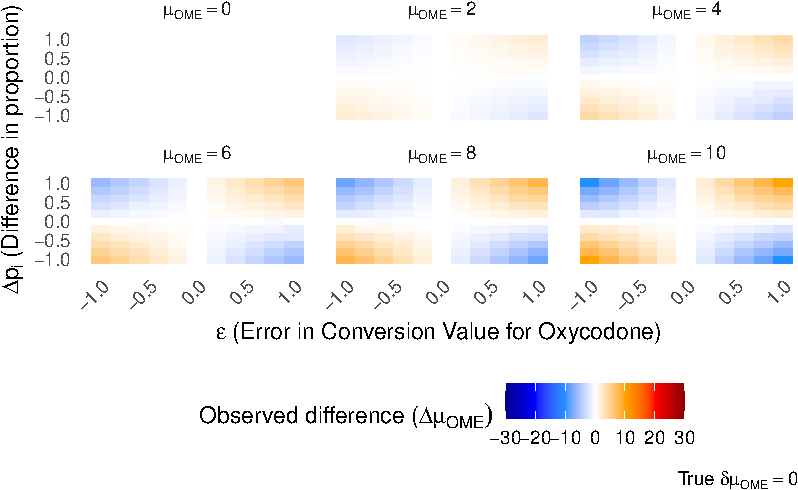
\includegraphics[keepaspectratio]{appendix_files/figure-pdf/fig-appendix-simple-sim-mu-1.pdf}}

}

\caption{\label{fig-appendix-simple-sim-mu}Plots of the difference in
proportion over the error in conversion values provided faceted by the
expected mean dose of the control group. Colour scale demonstrates the
observed difference in the treatment group. True effect size is set to
0.}

\end{figure}%

\subsection{\texorpdfstring{Effect of \(\Delta \mu_{\text{OME}}\) on
simple
simulation}{Effect of \textbackslash Delta \textbackslash mu\_\{\textbackslash text\{OME\}\} on simple simulation}}\label{sec-appendix-sim-2}

To investigate the interaction of a true treatment effect on the
observed treatment effect, 9 further simulations were performed, each as
described in Section~\ref{sec-manuscript-simple-sim} but with a
different true treatment effect between the values of -1 and 1.

\begin{figure}

\centering{

\pandocbounded{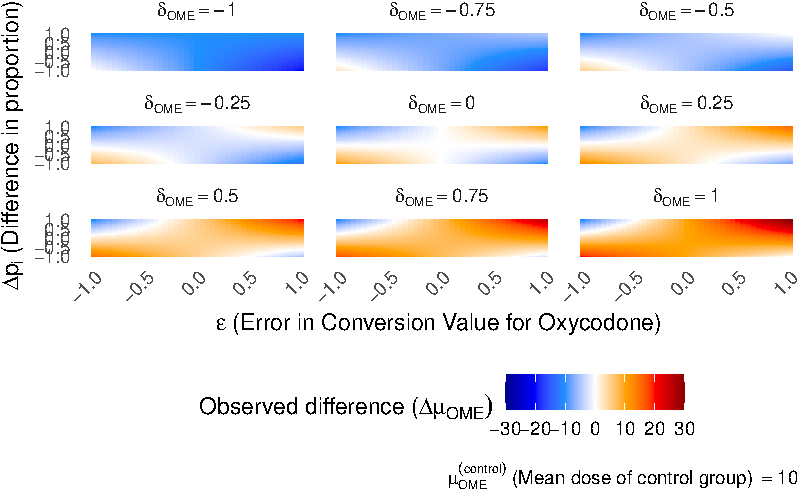
\includegraphics[keepaspectratio]{appendix_files/figure-pdf/fig-appendix-simple-sim-t-1.pdf}}

}

\caption{\label{fig-appendix-simple-sim-t}Plots of the difference in
proportion over the error in conversion values provided faceted by the
expected mean dose of the control group. Colour scale demonstrates the
observed difference in the treatment group. The mean value of the
control group is set to 10 OME mg .}

\end{figure}%

\subsection{Power calculation}\label{sec-appendix-simulation-power}

In the first part of the experiment a large effect size is used.

For a study period of 5.9904306 years and a annual case volume of 100
the total number of expected study participants is 599.0430622, of which
we would expect 239.5078606 to be robotic cases and 359.5352016 given a
2.9938483year period where 80\% of cases are performed robotically.

Assuming a 50 mg (SD: 10 mg) mean opioid requirement for the non-robotic
population, we can calculate the expected mean OME requirement for
robotic and non-robotic cases given a 0.8 effect size. The expected mean
OME requirement for robotic cases is 40 mg giving a mean difference of
-10 mg or -1 standard deviations.

Given the inital experimental set up it is clear that the study is very
highly powered with the power value to be calculated at 100\%.

Figure~\ref{fig-power-curve} demonstrated the power curve for the
comparison of OME between robotic and non-robotic surgical groups. The
dashed lines indicate the minimum detectable effect size at 80\% power.

\begin{figure}

\centering{

\pandocbounded{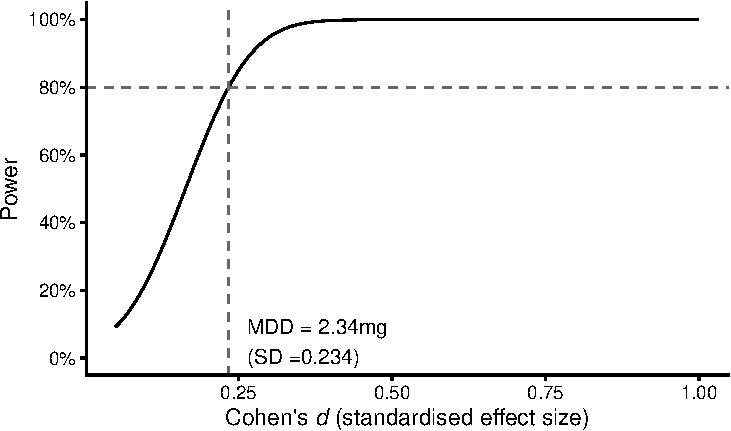
\includegraphics[keepaspectratio]{appendix_files/figure-pdf/fig-power-curve-1.pdf}}

}

\caption{\label{fig-power-curve}Power curve for the comparison of OME
between robotic and non-robotic surgical groups. The dashed lines
indicate the minimum detectable effect size at 80\% power.}

\end{figure}%

With the observed sample sizes, the minimum detectable effect size at
80\% power is \emph{d} = 0.234, which equates to a mean difference of
2.34 mg OME.

The effect size is use to inform the weakly powered study in

\begin{verbatim}


`<!-- quarto-file-metadata: eyJyZXNvdXJjZURpciI6Ii4ifQ== -->`{=html}

```{=html}
<!-- quarto-file-metadata: eyJyZXNvdXJjZURpciI6Ii4iLCJib29rSXRlbVR5cGUiOiJjaGFwdGVyIiwiYm9va0l0ZW1OdW1iZXIiOjIsImJvb2tJdGVtRmlsZSI6InNpbXVsYXRpb24ucW1kIiwiYm9va0l0ZW1EZXB0aCI6MX0= -->
\end{verbatim}

\chapter{Code for simulation study}\label{sec-sim}

\section{Code repository}\label{code-repository}

The code will be hosted on a public github.

\section{Simple simulation}\label{sec-sim-simple}

The \texttt{sim\_simple} function simulates a simple experiment with two
equally groups, control and treatment, for total \texttt{n} samples.
\texttt{delta\_p\_i} controls the difference in proportion of
medications \texttt{i} between the two groups. For each patient a
expected opioid requirement is sampled from a normal distribution with
mean \texttt{mu\_opioid\_requirment\_control} and standard deviation
\texttt{sigma}. The treatment group has a mean opioid requirement that
is increased by the factor of \texttt{treatment\_effect}. For samples
where \texttt{i} is \texttt{"oxycodone"}, the expected opioid
requirement is converted to a oxycodone dose using
\texttt{potency\_oxycodone} and then converted back into expected dose
of morphine (the OME) using the conversion factor
\texttt{potency\_oxycodone} +/- an error term
\texttt{error\_in\_c\_oxycodone}.

The function then returns the difference between the OME dose between
the control and treatment group.

\begin{Shaded}
\begin{Highlighting}[]
\NormalTok{sim\_simple }\OtherTok{\textless{}{-}} \ControlFlowTok{function}\NormalTok{(n, }\CommentTok{\# total number of patients}
\NormalTok{                       delta\_p\_i, }\CommentTok{\# Difference in proportion of i between groups,}
                       \AttributeTok{i =} \FunctionTok{c}\NormalTok{(}\StringTok{"morphine"}\NormalTok{, }\StringTok{"oxycodone"}\NormalTok{), }\CommentTok{\# The two medications}
                       \AttributeTok{mu\_opioid\_requirment\_control =} \DecValTok{1}\NormalTok{, }
                       \AttributeTok{sigma =} \FloatTok{0.1}\NormalTok{,}
                       \AttributeTok{treatment\_effect =} \DecValTok{0}\NormalTok{,}
\NormalTok{                       potency\_oxycodone,}
                       \AttributeTok{error\_in\_c\_oxycodone =} \DecValTok{0}\NormalTok{)\{}
  
\NormalTok{   group\_control }\OtherTok{=} \FunctionTok{data.frame}\NormalTok{(}
     \AttributeTok{group =} \StringTok{"control"}\NormalTok{,}
     \AttributeTok{drug =} \FunctionTok{sample}\NormalTok{(i, }\AttributeTok{size =}\NormalTok{ n}\SpecialCharTok{/}\DecValTok{2}\NormalTok{, }\AttributeTok{replace =} \ConstantTok{TRUE}\NormalTok{, }\AttributeTok{prob =} \FunctionTok{c}\NormalTok{(}\FloatTok{0.5}\SpecialCharTok{+}\NormalTok{delta\_p\_i}\SpecialCharTok{/}\DecValTok{2}\NormalTok{, }\FloatTok{0.5}\SpecialCharTok{{-}}\NormalTok{delta\_p\_i}\SpecialCharTok{/}\DecValTok{2}\NormalTok{)),}
     \AttributeTok{opioid\_req =} \FunctionTok{rnorm}\NormalTok{(n}\SpecialCharTok{/}\DecValTok{2}\NormalTok{, }\AttributeTok{mean =}\NormalTok{ mu\_opioid\_requirment\_control, }\AttributeTok{sd =}\NormalTok{ sigma)}
\NormalTok{   )}
  
\NormalTok{  group\_treatment }\OtherTok{=} \FunctionTok{data.frame}\NormalTok{(}
     \AttributeTok{group =} \StringTok{"treatment"}\NormalTok{,}
     \AttributeTok{drug =} \FunctionTok{sample}\NormalTok{(i, }\AttributeTok{size =}\NormalTok{ n}\SpecialCharTok{/}\DecValTok{2}\NormalTok{, }\AttributeTok{replace =} \ConstantTok{TRUE}\NormalTok{, }\AttributeTok{prob =} \FunctionTok{c}\NormalTok{(}\FloatTok{0.5}\SpecialCharTok{{-}}\NormalTok{delta\_p\_i}\SpecialCharTok{/}\DecValTok{2}\NormalTok{, }\FloatTok{0.5}\SpecialCharTok{+}\NormalTok{delta\_p\_i}\SpecialCharTok{/}\DecValTok{2}\NormalTok{)),}
     \AttributeTok{opioid\_req =} \FunctionTok{rnorm}\NormalTok{(n}\SpecialCharTok{/}\DecValTok{2}\NormalTok{, }\AttributeTok{mean =}\NormalTok{ mu\_opioid\_requirment\_control}\SpecialCharTok{+}\NormalTok{(mu\_opioid\_requirment\_control}\SpecialCharTok{*}\NormalTok{treatment\_effect), }\AttributeTok{sd =}\NormalTok{ sigma)}
\NormalTok{   )}
  
\NormalTok{  result }\OtherTok{\textless{}{-}} \FunctionTok{rbind}\NormalTok{(group\_control,group\_treatment) }\SpecialCharTok{\%\textgreater{}\%}
    \FunctionTok{mutate}\NormalTok{(}\AttributeTok{dose\_recived =} \FunctionTok{ifelse}\NormalTok{(drug }\SpecialCharTok{==} \StringTok{"morphine"}\NormalTok{, opioid\_req, opioid\_req}\SpecialCharTok{/}\NormalTok{potency\_oxycodone),}
           \AttributeTok{ome =} \FunctionTok{ifelse}\NormalTok{(drug }\SpecialCharTok{==} \StringTok{"morphine"}\NormalTok{, dose\_recived, dose\_recived}\SpecialCharTok{*}\NormalTok{(potency\_oxycodone}\SpecialCharTok{+}\NormalTok{(potency\_oxycodone}\SpecialCharTok{*}\NormalTok{error\_in\_c\_oxycodone))}
\NormalTok{                        ))}
  
\NormalTok{  analysis }\OtherTok{\textless{}{-}}\NormalTok{ result }\SpecialCharTok{\%\textgreater{}\%}
    \FunctionTok{group\_by}\NormalTok{(group) }\SpecialCharTok{\%\textgreater{}\%}
    \FunctionTok{summarise}\NormalTok{(}\AttributeTok{proportion\_morphine =} \FunctionTok{sum}\NormalTok{(drug }\SpecialCharTok{==} \StringTok{"morphine"}\NormalTok{)}\SpecialCharTok{/}\FunctionTok{n}\NormalTok{(),}
              \AttributeTok{mean\_ome =} \FunctionTok{mean}\NormalTok{(ome),}
              \AttributeTok{n =} \FunctionTok{n}\NormalTok{(),}
              \AttributeTok{.groups =} \StringTok{"drop"}\NormalTok{) }
    
  \FunctionTok{return}\NormalTok{(analysis}\SpecialCharTok{$}\NormalTok{mean\_ome[}\DecValTok{2}\NormalTok{] }\SpecialCharTok{{-}}\NormalTok{ analysis}\SpecialCharTok{$}\NormalTok{mean\_ome[}\DecValTok{1}\NormalTok{])}
  
\NormalTok{\}}
\end{Highlighting}
\end{Shaded}

\section{Exemplar simulation}\label{sec-sim-exemplar}

The \texttt{sim\_patient} function produces a study dataset by seeding
procedure dates given the annual case load and the study period. Then
for each procedure sampling whether the procedure is robotic or
standard, and finally sampling which opioid is used.

The function then estimates the mean analgesia requirement based on
treatment and opioid and samples the dose from a normal distribution.

\begin{Shaded}
\begin{Highlighting}[]
\NormalTok{sim\_patient }\OtherTok{\textless{}{-}} \ControlFlowTok{function}\NormalTok{(}
  \AttributeTok{mu\_tot =} \DecValTok{50}\NormalTok{,}
  \AttributeTok{potency\_oxycodone\_truth =} \FloatTok{1.85}\NormalTok{,}
  \AttributeTok{potency\_oxycodone\_ome =} \DecValTok{2}\NormalTok{,}
  \AttributeTok{proportion\_morphine =} \FloatTok{0.7}\NormalTok{,}
  \AttributeTok{oxycodone\_shortage =} \FunctionTok{c}\NormalTok{(}\FunctionTok{as.Date}\NormalTok{(}\StringTok{"2024{-}01{-}01"}\NormalTok{), }\FunctionTok{as.Date}\NormalTok{(}\StringTok{"2024{-}12{-}31"}\NormalTok{)),}
  \AttributeTok{t\_0 =} \FunctionTok{as.Date}\NormalTok{(}\StringTok{"2020{-}01{-}01"}\NormalTok{),}
  \AttributeTok{t\_end =} \FunctionTok{as.Date}\NormalTok{(}\StringTok{"2025{-}12{-}31"}\NormalTok{),}
  \AttributeTok{t\_robot =} \FunctionTok{as.Date}\NormalTok{(}\StringTok{"2023{-}01{-}01"}\NormalTok{),}
  \AttributeTok{annual\_n =} \DecValTok{30}\NormalTok{,}
  \AttributeTok{robot\_effect\_size =} \FloatTok{0.8}
\NormalTok{)\{}
  \CommentTok{\# Calculate total number of patients over the study period}
\NormalTok{  total\_days }\OtherTok{\textless{}{-}} \FunctionTok{as.numeric}\NormalTok{(t\_end }\SpecialCharTok{{-}}\NormalTok{ t\_0)}
\NormalTok{  total\_years }\OtherTok{\textless{}{-}}\NormalTok{ total\_days }\SpecialCharTok{/} \FloatTok{365.25}
\NormalTok{  total\_n }\OtherTok{\textless{}{-}} \FunctionTok{round}\NormalTok{(total\_years }\SpecialCharTok{*}\NormalTok{ annual\_n)}

  \CommentTok{\# Sample random dates}
\NormalTok{  dates }\OtherTok{\textless{}{-}} \FunctionTok{as.Date}\NormalTok{(}\FunctionTok{runif}\NormalTok{(total\_n, }\AttributeTok{min =} \FunctionTok{as.numeric}\NormalTok{(t\_0), }\AttributeTok{max =} \FunctionTok{as.numeric}\NormalTok{(t\_end)), }\AttributeTok{origin =} \StringTok{"1970{-}01{-}01"}\NormalTok{)}

  \CommentTok{\# Sample if procedure is robotic (after 2023, 80\% chance)}
\NormalTok{  robotic }\OtherTok{\textless{}{-}} \FunctionTok{ifelse}\NormalTok{(dates }\SpecialCharTok{\textgreater{}=}\NormalTok{ t\_robot, }\FunctionTok{rbinom}\NormalTok{(total\_n, }\DecValTok{1}\NormalTok{, }\FloatTok{0.8}\NormalTok{) }\SpecialCharTok{==} \DecValTok{1}\NormalTok{, }\ConstantTok{FALSE}\NormalTok{)}

  \CommentTok{\# Sample which opioid is used}
  \CommentTok{\# During 2024, 100\% morphine. Otherwise, 40\% oxycodone, 60\% morphine.}
\NormalTok{  is\_shortage }\OtherTok{\textless{}{-}}\NormalTok{ dates }\SpecialCharTok{\textgreater{}=}\NormalTok{ oxycodone\_shortage[}\DecValTok{1}\NormalTok{] }\SpecialCharTok{\&}\NormalTok{ dates }\SpecialCharTok{\textless{}=}\NormalTok{ oxycodone\_shortage[}\DecValTok{2}\NormalTok{]}
\NormalTok{  opioid }\OtherTok{\textless{}{-}} \FunctionTok{ifelse}\NormalTok{(is\_shortage, }\StringTok{"M"}\NormalTok{,}
    \FunctionTok{ifelse}\NormalTok{(}\FunctionTok{rbinom}\NormalTok{(total\_n, }\DecValTok{1}\NormalTok{, proportion\_morphine) }\SpecialCharTok{==} \DecValTok{1}\NormalTok{, }\StringTok{"M"}\NormalTok{, }\StringTok{"O"}\NormalTok{)}
\NormalTok{  )}

  \CommentTok{\# Estimate mean analgesia requirement based on treatment}
\NormalTok{  mu }\OtherTok{\textless{}{-}} \FunctionTok{ifelse}\NormalTok{(robotic, mu\_tot }\SpecialCharTok{*}\NormalTok{ robot\_effect\_size, mu\_tot)}

  \CommentTok{\# Set mean dose depending on opioid type (using true potency)}
\NormalTok{  mu\_op }\OtherTok{\textless{}{-}} \FunctionTok{ifelse}\NormalTok{(opioid }\SpecialCharTok{==} \StringTok{"M"}\NormalTok{, mu, mu }\SpecialCharTok{/}\NormalTok{ potency\_oxycodone\_truth)}

  \CommentTok{\# Sample dose from normal distribution}
\NormalTok{  dose }\OtherTok{\textless{}{-}} \FunctionTok{rnorm}\NormalTok{(total\_n, }\AttributeTok{mean =}\NormalTok{ mu\_op, }\AttributeTok{sd =} \DecValTok{10}\NormalTok{)}

  \CommentTok{\# Round the doses to an integer of milligrams and prevent negative doses}
\NormalTok{  dose }\OtherTok{\textless{}{-}} \FunctionTok{pmax}\NormalTok{(}\DecValTok{0}\NormalTok{, }\FunctionTok{round}\NormalTok{(dose))}

  \CommentTok{\# Create final dataframe}
\NormalTok{  df }\OtherTok{\textless{}{-}} \FunctionTok{data.frame}\NormalTok{(}
    \AttributeTok{date =}\NormalTok{ dates,}
    \AttributeTok{robotic =}\NormalTok{ robotic,}
    \AttributeTok{opioid =}\NormalTok{ opioid,}
    \AttributeTok{dose =}\NormalTok{ dose}
\NormalTok{  )}

  \CommentTok{\# Sort by date for chronological sense}
\NormalTok{  df }\OtherTok{\textless{}{-}}\NormalTok{ df[}\FunctionTok{order}\NormalTok{(df}\SpecialCharTok{$}\NormalTok{date), ]}
  \FunctionTok{rownames}\NormalTok{(df) }\OtherTok{\textless{}{-}} \ConstantTok{NULL}
  
\NormalTok{  df }\OtherTok{\textless{}{-}}\NormalTok{ df }\SpecialCharTok{\%\textgreater{}\%}
      \FunctionTok{mutate}\NormalTok{(}\AttributeTok{ome =} \FunctionTok{case\_when}\NormalTok{(}
\NormalTok{        opioid }\SpecialCharTok{==} \StringTok{"M"} \SpecialCharTok{\textasciitilde{}}\NormalTok{ dose,}
\NormalTok{        opioid }\SpecialCharTok{==} \StringTok{"O"} \SpecialCharTok{\textasciitilde{}}\NormalTok{ dose }\SpecialCharTok{*} \DecValTok{1}\SpecialCharTok{*}\NormalTok{potency\_oxycodone\_ome}
\NormalTok{      ))}
 
\NormalTok{  df }\OtherTok{\textless{}{-}}\NormalTok{ df }\SpecialCharTok{\%\textgreater{}\%} \FunctionTok{mutate}\NormalTok{(}
    \AttributeTok{robotic =} \FunctionTok{factor}\NormalTok{(robotic, }\AttributeTok{labels =} \FunctionTok{c}\NormalTok{(}\StringTok{"Non{-}Robotic"}\NormalTok{, }\StringTok{"Robotic"}\NormalTok{)),}
    \AttributeTok{opioid =} \FunctionTok{factor}\NormalTok{(opioid, }\AttributeTok{levels =} \FunctionTok{c}\NormalTok{(}\StringTok{"M"}\NormalTok{, }\StringTok{"O"}\NormalTok{), }\AttributeTok{labels =} \FunctionTok{c}\NormalTok{(}\StringTok{"Morphine"}\NormalTok{, }\StringTok{"Oxycodone"}\NormalTok{))}
\NormalTok{  )}

  \FunctionTok{return}\NormalTok{(df)}
\NormalTok{\}}
\end{Highlighting}
\end{Shaded}

The \texttt{analyse\_dataset} function acts to hypothesis test the
difference in mean OME between robotic and non-robotic procedures.

\begin{Shaded}
\begin{Highlighting}[]
\NormalTok{analyse\_dataset }\OtherTok{\textless{}{-}} \ControlFlowTok{function}\NormalTok{(df)\{}
  \CommentTok{\# Perform t{-}test for difference in mean OME between robotic and non{-}robotic procedures}
\NormalTok{  t\_test\_result }\OtherTok{\textless{}{-}} \FunctionTok{t.test}\NormalTok{(ome }\SpecialCharTok{\textasciitilde{}}\NormalTok{ robotic, }\AttributeTok{data =}\NormalTok{ df)}

  \CommentTok{\# analyse the difference between the opioid proportions}
\NormalTok{  fishers\_result }\OtherTok{\textless{}{-}} \FunctionTok{fisher.test}\NormalTok{(}\FunctionTok{table}\NormalTok{(df}\SpecialCharTok{$}\NormalTok{robotic, df}\SpecialCharTok{$}\NormalTok{opioid)) }
  
  \CommentTok{\# Return results as a list}
  \FunctionTok{return}\NormalTok{(}\FunctionTok{list}\NormalTok{(}
    \AttributeTok{mean\_diff\_ome =} \FunctionTok{diff}\NormalTok{(t\_test\_result}\SpecialCharTok{$}\NormalTok{estimate),}
    \AttributeTok{p\_value\_ome =}\NormalTok{ t\_test\_result}\SpecialCharTok{$}\NormalTok{p.value,}
    \AttributeTok{conf\_int\_ome =}\NormalTok{ t\_test\_result}\SpecialCharTok{$}\NormalTok{conf.int,}
    \AttributeTok{chisq\_result\_medication =}\NormalTok{ fishers\_result}\SpecialCharTok{$}\NormalTok{p.value}
\NormalTok{  ))}
\NormalTok{\}}
\end{Highlighting}
\end{Shaded}

The \texttt{run\ simulation} function will run \(t\) trials for each of
the values of the conversion values \(c_{\text{Oxycodone}}\) and the
proportion of morphine perceribed post-operativly. The results will be
stored in a data frame and then summarized using the mean of the results
of the \texttt{analyse\_dataset} function.

\begin{Shaded}
\begin{Highlighting}[]
\NormalTok{run\_simulation }\OtherTok{\textless{}{-}} \ControlFlowTok{function}\NormalTok{(}\AttributeTok{trials =} \DecValTok{5}\NormalTok{,}
                          \AttributeTok{conversion\_values =} \FunctionTok{seq}\NormalTok{(}\AttributeTok{from=}\DecValTok{1}\NormalTok{, }\AttributeTok{to=}\DecValTok{4}\NormalTok{, }\AttributeTok{by =} \FloatTok{0.2}\NormalTok{),}
                          \AttributeTok{morphine\_proportion =} \FunctionTok{seq}\NormalTok{(}\AttributeTok{from =}\FloatTok{0.1}\NormalTok{, }\AttributeTok{to=} \FloatTok{0.9}\NormalTok{, }\AttributeTok{by =} \FloatTok{0.05}\NormalTok{))}
\NormalTok{                          \{}

  \ControlFlowTok{for}\NormalTok{(t }\ControlFlowTok{in} \DecValTok{1}\SpecialCharTok{:}\NormalTok{trials)\{}
    \ControlFlowTok{for}\NormalTok{(i }\ControlFlowTok{in}\NormalTok{ conversion\_values)\{}
      \ControlFlowTok{for}\NormalTok{(j }\ControlFlowTok{in}\NormalTok{ morphine\_proportion)\{}
    
\NormalTok{    df }\OtherTok{\textless{}{-}} \FunctionTok{sim\_patient}\NormalTok{(}
      \AttributeTok{mu\_tot =}\NormalTok{ mu\_tot,}
      \AttributeTok{potency\_oxycodone\_truth =}\NormalTok{ potency\_oxycodone\_truth,}
      \AttributeTok{potency\_oxycodone\_ome =}\NormalTok{ i,}
      \AttributeTok{proportion\_morphine =}\NormalTok{ j,}
      \AttributeTok{oxycodone\_shortage =}\NormalTok{ oxycodone\_shortage,}
      \AttributeTok{t\_0 =}\NormalTok{ t\_0,}
      \AttributeTok{t\_end =}\NormalTok{ t\_end,}
      \AttributeTok{t\_robot =}\NormalTok{ t\_robot,}
      \AttributeTok{annual\_n =}\NormalTok{ annual\_n,}
      \AttributeTok{robot\_effect\_size =}\NormalTok{ robot\_effect\_size}
\NormalTok{    )}
    
\NormalTok{    delta\_p\_oxycodone }\OtherTok{\textless{}{-}}\NormalTok{ df }\SpecialCharTok{|\textgreater{}}
      \FunctionTok{group\_by}\NormalTok{(robotic) }\SpecialCharTok{|\textgreater{}}
      \FunctionTok{summarise}\NormalTok{(}\AttributeTok{p =} \FunctionTok{mean}\NormalTok{(opioid }\SpecialCharTok{==} \StringTok{"Oxycodone"}\NormalTok{)) }\SpecialCharTok{|\textgreater{}}
      \FunctionTok{pull}\NormalTok{(p) }\SpecialCharTok{|\textgreater{}}
      \FunctionTok{diff}\NormalTok{()}
    
\NormalTok{    epsilon }\OtherTok{\textless{}{-}}\NormalTok{ (i }\SpecialCharTok{{-}}\NormalTok{ potency\_oxycodone\_truth)}\SpecialCharTok{/}\NormalTok{potency\_oxycodone\_truth}
    
    
\NormalTok{    result }\OtherTok{\textless{}{-}} \FunctionTok{analyse\_dataset}\NormalTok{(df)}
    
    \ControlFlowTok{if}\NormalTok{(t }\SpecialCharTok{==} \DecValTok{1} \SpecialCharTok{\&}\NormalTok{ i }\SpecialCharTok{==}\NormalTok{ conversion\_values[}\DecValTok{1}\NormalTok{] }\SpecialCharTok{\&}\NormalTok{ j }\SpecialCharTok{==}\NormalTok{ morphine\_proportion[}\DecValTok{1}\NormalTok{])\{}
      
\NormalTok{      results\_grid }\OtherTok{\textless{}{-}} \FunctionTok{data.frame}\NormalTok{(}
        \AttributeTok{trial =}\NormalTok{ t,}
        \AttributeTok{conversion\_value =}\NormalTok{ i,}
        \AttributeTok{morphine\_proportion =}\NormalTok{ j,}
        \AttributeTok{mean\_diff\_ome =}\NormalTok{ result}\SpecialCharTok{$}\NormalTok{mean\_diff\_ome,}
        \AttributeTok{p\_value\_ome =}\NormalTok{ result}\SpecialCharTok{$}\NormalTok{p\_value\_ome,}
        \AttributeTok{p\_value\_fishers =}\NormalTok{ result}\SpecialCharTok{$}\NormalTok{chisq\_result\_medication,}
        \AttributeTok{delta\_p\_oxycodone =}\NormalTok{ delta\_p\_oxycodone,}
        \AttributeTok{epsilon =}\NormalTok{ epsilon}
\NormalTok{      )}
\NormalTok{    \}}\ControlFlowTok{else}\NormalTok{\{}
    \CommentTok{\# Store results}
\NormalTok{    results\_grid }\OtherTok{\textless{}{-}} \FunctionTok{rbind}\NormalTok{(results\_grid, }\FunctionTok{data.frame}\NormalTok{(}
      \AttributeTok{trial=}\NormalTok{t,}
      \AttributeTok{conversion\_value =}\NormalTok{ i,}
      \AttributeTok{morphine\_proportion =}\NormalTok{ j,}
      \AttributeTok{mean\_diff\_ome =}\NormalTok{ result}\SpecialCharTok{$}\NormalTok{mean\_diff\_ome,}
      \AttributeTok{p\_value\_ome =}\NormalTok{ result}\SpecialCharTok{$}\NormalTok{p\_value\_ome,}
      \AttributeTok{p\_value\_fishers =}\NormalTok{ result}\SpecialCharTok{$}\NormalTok{chisq\_result\_medication,}
      \AttributeTok{delta\_p\_oxycodone =}\NormalTok{ delta\_p\_oxycodone,}
      \AttributeTok{epsilon =}\NormalTok{ epsilon}
\NormalTok{    ))}
\NormalTok{    \}}
    
\NormalTok{  \}}
\NormalTok{  \}}
\NormalTok{\}}

\NormalTok{  results\_grid }\OtherTok{\textless{}{-}}\NormalTok{ results\_grid }\SpecialCharTok{\%\textgreater{}\%} \FunctionTok{group\_by}\NormalTok{(conversion\_value, morphine\_proportion) }\SpecialCharTok{\%\textgreater{}\%}
    \FunctionTok{summarise}\NormalTok{(}\AttributeTok{mean\_diff\_ome =} \FunctionTok{mean}\NormalTok{(mean\_diff\_ome),}
            \AttributeTok{p\_value\_ome =} \FunctionTok{mean}\NormalTok{(p\_value\_ome),}
            \AttributeTok{p\_value\_fishers =} \FunctionTok{mean}\NormalTok{(p\_value\_fishers),}
            \AttributeTok{delta\_p\_oxycodone =} \FunctionTok{mean}\NormalTok{(delta\_p\_oxycodone),}
            \AttributeTok{epsilon =} \FunctionTok{mean}\NormalTok{(epsilon),}
            \AttributeTok{.groups =} \StringTok{"drop"}\NormalTok{) }\SpecialCharTok{\%\textgreater{}\%}
    \FunctionTok{mutate}\NormalTok{(}\AttributeTok{significant =} \FunctionTok{ifelse}\NormalTok{(p\_value\_ome }\SpecialCharTok{\textless{}} \FloatTok{0.05}\NormalTok{, }\StringTok{"*"}\NormalTok{, }\StringTok{""}\NormalTok{))}

  \FunctionTok{return}\NormalTok{(results\_grid)}

\NormalTok{\} }
\end{Highlighting}
\end{Shaded}

\texttt{plot\_grid()} function plots the heatmap of the results of the
exemplar simulation.

\begin{Shaded}
\begin{Highlighting}[]
\NormalTok{plot\_grid }\OtherTok{\textless{}{-}} \ControlFlowTok{function}\NormalTok{(results\_grid,}
\NormalTok{                      potency\_oxycodone\_truth,}
\NormalTok{                      robot\_effect\_mg)\{}

\NormalTok{midpoint }\OtherTok{\textless{}{-}}\NormalTok{ robot\_effect\_mg}
\NormalTok{min\_val }\OtherTok{\textless{}{-}} \FunctionTok{min}\NormalTok{(results\_grid}\SpecialCharTok{$}\NormalTok{mean\_diff\_ome, }\AttributeTok{na.rm =} \ConstantTok{TRUE}\NormalTok{)  }\CommentTok{\# adjust column name as needed}
\NormalTok{max\_val }\OtherTok{\textless{}{-}} \FunctionTok{max}\NormalTok{(results\_grid}\SpecialCharTok{$}\NormalTok{mean\_diff\_ome, }\AttributeTok{na.rm =} \ConstantTok{TRUE}\NormalTok{)}

 \FunctionTok{ggplot}\NormalTok{(results\_grid, }\FunctionTok{aes}\NormalTok{(}\AttributeTok{x=}\NormalTok{conversion\_value, }\AttributeTok{y=}\NormalTok{morphine\_proportion, }\AttributeTok{fill=}\NormalTok{mean\_diff\_ome)) }\SpecialCharTok{+}
  \FunctionTok{geom\_tile}\NormalTok{() }\SpecialCharTok{+}
  \FunctionTok{geom\_text}\NormalTok{(}\FunctionTok{aes}\NormalTok{(}\AttributeTok{label =}\NormalTok{ significant), }\AttributeTok{color =} \StringTok{"darkgreen"}\NormalTok{) }\SpecialCharTok{+}
  \FunctionTok{scale\_fill\_gradientn}\NormalTok{(}
  \AttributeTok{colours =} \FunctionTok{c}\NormalTok{(}\StringTok{"blue"}\NormalTok{, }\StringTok{"dodgerblue"}\NormalTok{, }\StringTok{"white"}\NormalTok{, }\StringTok{"orange"}\NormalTok{, }\StringTok{"red"}\NormalTok{),}
  \AttributeTok{values =}\NormalTok{ scales}\SpecialCharTok{::}\FunctionTok{rescale}\NormalTok{(}\FunctionTok{c}\NormalTok{(}
\NormalTok{    min\_val,}
\NormalTok{    (min\_val }\SpecialCharTok{+}\NormalTok{ midpoint) }\SpecialCharTok{/} \DecValTok{2}\NormalTok{,}
\NormalTok{    midpoint,}
\NormalTok{    (midpoint }\SpecialCharTok{+}\NormalTok{ max\_val) }\SpecialCharTok{/} \DecValTok{2}\NormalTok{,}
\NormalTok{    max\_val}
\NormalTok{  )),}
  \AttributeTok{limits =} \FunctionTok{c}\NormalTok{(min\_val, max\_val)}
\NormalTok{)}\SpecialCharTok{+}
  \FunctionTok{labs}\NormalTok{(}\AttributeTok{title =}\NormalTok{ ,}
       \AttributeTok{x =} \StringTok{"$c\_\{}\SpecialCharTok{\textbackslash{}t}\StringTok{ext\{Oxycodone\}\}$"}\NormalTok{,}
       \AttributeTok{y =} \StringTok{"Proportion of Morphine"}\NormalTok{,}
       \AttributeTok{fill =} \StringTok{"Mean Difference in OME"}\NormalTok{,}
       \AttributeTok{caption =} \StringTok{"Blue * denotes significant testing with p value \textless{} 0.05"}\NormalTok{) }\SpecialCharTok{+}
   \FunctionTok{geom\_vline}\NormalTok{(}\AttributeTok{xintercept =}\NormalTok{ potency\_oxycodone\_truth, }\AttributeTok{linetype =} \StringTok{"dashed"}\NormalTok{, }\AttributeTok{color =} \StringTok{"red"}\NormalTok{)}\SpecialCharTok{+}
  \FunctionTok{theme\_minimal}\NormalTok{() }\SpecialCharTok{+}
  \FunctionTok{theme}\NormalTok{(}
    \AttributeTok{axis.text.x =} \FunctionTok{element\_text}\NormalTok{(}\AttributeTok{angle =} \DecValTok{45}\NormalTok{, }\AttributeTok{hjust =} \DecValTok{1}\NormalTok{),}
    \AttributeTok{panel.grid =} \FunctionTok{element\_blank}\NormalTok{(),}
    \AttributeTok{legend.position =} \StringTok{"bottom"}
\NormalTok{  )}
 
\NormalTok{\}}
\end{Highlighting}
\end{Shaded}

\texttt{symetic\_fill\_scale} is a colour gradient scale that allows
control of the scale to ensure consistancy between plots




\end{document}
